\documentclass{article}
\usepackage{graphicx}
\usepackage{xcolor}
\usepackage[utf8]{inputenc}
\usepackage[T1]{fontenc}
\renewcommand{\rmdefault}{ptm}
\renewcommand{\sfdefault}{ptm}
\renewcommand{\ttdefault}{ptm}
\usepackage[french]{babel}
\usepackage{textcomp}
% Si vous voulez réinitialiser la numérotation des sections et pages à un certain point
\usepackage{titlesec}
\usepackage{url}
\usepackage{ragged2e}
\usepackage{enumitem}
\usepackage[a4paper, margin=2.5cm]{geometry}  % Ajuster les marges à 2.5 cm de chaque côté
\renewcommand{\thesection}{\arabic{section}} % Utiliser des chiffres arabes pour la numérotation des sections

\begin{document}
% Page de couverture
\begin{titlepage}
    \centering
    
\includegraphics[width=0.4\textwidth]{ressources/logoSorbonne.png}
    \begin{center}
        \hrulefill \\[1cm]
        \Huge\textbf{Sorbonne Université} \\[1cm]
        \Large\textbf{Master 2 Science et Technologie du Logiciel} \\ [1cm]
        \hrulefill \\[2cm]
        \huge\textbf{Rapport du projet 1 DAAR : Automate } \\[1cm]
        \huge\textbf{\textcolor{cyan}{Clone de egrep avec support partiel des ERE}} \\[2cm]
        \hrulefill \\[2.5cm]
        \Large\textbf{Auteurs:} Florian CODEBECQ, Nandraina RAZAFINDRAIBE\\[1cm] 
        \Large\textbf{Responsable:} Binh-Minh BUI-XUAN\\[2.5cm]
        \textbf{Année scolaire:} 2024/2025  
    \end{center}
\end{titlepage}

% Page suivant %
\newpage

\tableofcontents

\newpage

\setcounter{page}{1}

\setcounter{section}{0}
\section{Introduction}
Dans ce projet, nous avons développé un clone partiel de la commande Linux egrep, capable de rechercher des motifs dans un fichier textuel à l'aide d'expressions régulières étendues (ERE). L'objectif principal est d'explorer plusieurs approches d'implémentation des algorithmes de recherche de motifs, et d'analyser leurs performances.

Pour la réalisation du projet, nous avons décidé d'utiliser Java comme langage de programmation.

\section{Problématique et Objectifs}
Le problème à résoudre est la recherche de motifs dans des fichiers textuels en utilisant des expressions régulières conformes à la norme ERE. Deux stratégies principales sont considérées :

\begin{itemize}
    \item Automates : Transformation de l'expression régulière en automate fini non déterministe (AFND) avec $\epsilon$-transitions, puis en automate fini déterministe (AFD) via la méthode des sous-ensembles.
    \item Recherche linéaire : Utilisation de l'algorithme Knuth-Morris-Pratt (KMP) pour la recherche de motifs simples.
\end{itemize}

\section{Méthodologie}
\subsection{Méthode d’Aho-Ullman}
L’algorithme Aho-Ullman est une méthode efficace pour effectuer  une recherche simultanée de plusieurs  motifs dans un texte.

Cette approche consiste à construire un automate fini à partir d’une expression régulière. Pour parvenir à notre objectif, on doit passer sur plusieurs étapes:
\begin{itemize}
    \item Construction d'un arbre syntaxique à partir d’\textbf{une expression régulière}.
    \item Conversion de cet arbre en \textbf{un automate fini non déterministe (AFND)} avec $\epsilon$-transition.
    \item Transformer de l’automate fini non déterministe en \textbf{un automate fini déterministe (AFD)}.
    \item Optimiser l’AFD afin d’obtenir un automate avec un nombre minimum d’états.
    \item Rechercher les motifs avec l’automate ainsi obtenu.
\end{itemize}

\subsubsection{Une expression régulière vers l’arbre syntaxique}
Cette étape réalise une analyse syntaxique du motif entré par l'utilisateur en identifiant les opérations à effectuer sur les caractères qui le composent. Les opérations respectent l'ordre de priorité suivant : les parenthèses "()", les quantificateurs "*", la concaténation ".", et l'alternance "|".

Pour ce projet, un code en Java a été fourni dès le départ, qui prend en entrée une expression régulière et retourne l'arbre syntaxique correspondant. Nous avons ensuite basé la suite du projet sur ce code.
\subsubsection{Construire l’automate fini non déterministe}
Nous devons définir des règles pour chaque opération dans l'arbre syntaxique afin de les combiner et, en fin de compte, générer l'automate correspondant. Pour clarifier ce processus, prenons l'exemple de l'arbre " .(a,b)".

Ci-dessous, nous montrons l'équivalence entre sa représentation en graphe et son équivalent sous forme de tableau. Lors de la transformation en automate, chaque lettre est représentée par un minimum de 4 états.

\begin{figure}[h]
    \begin{minipage}{0.3\textwidth}
        \centering
        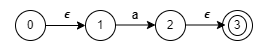
\includegraphics[width=\textwidth]{ressources/NDFA_a.png}
        \caption{Automate fini non déterministe de "a"}
        \label{fig:ndfa_a}
        \cite{ndfa_a}
    \end{minipage}
    \hspace{5cm} % Espace horizontal entre les deux images
    \begin{minipage}{0.25\textwidth}
        \centering
        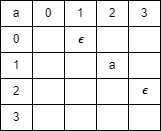
\includegraphics[width=\textwidth]{ressources/NDFA_a.tab.png}
        \caption{Représentation sous forme de tableau de "a"}
        \label{fig:ndfa_tab_a}
        \cite{ndfa_tab_a}
    \end{minipage}
\end{figure}

\newpage
\begin{figure}[h]
    \begin{minipage}{0.3\textwidth}
        \centering
        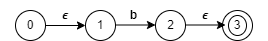
\includegraphics[width=\textwidth]{ressources/NDFA_b.png}
        \caption{Automate fini non déterministe de "b"}
        \label{fig:ndfa_b}
        \cite{ndfa_b}
    \end{minipage}
    \hspace{5cm} % Espace horizontal entre les deux images
    \begin{minipage}{0.25\textwidth}
        \centering
        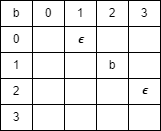
\includegraphics[width=\textwidth]{ressources/NDFA_b.tab.png}
        \caption{Représentation sous forme de tableau de "b"}
        \label{fig:ndfa_tab_b}
        \cite{ndfa_tab_b}
    \end{minipage}
\end{figure}

Cette étape consiste à remonter dans l'arbre tout en combinant les feuilles, en commençant par le niveau le plus profond. Les opérations indiquées sur les nœuds dictent les règles à suivre pour effectuer la combinaison.

\begin{figure}[h] % Utilisation de l'option [h] pour placer l'image ici
    \centering
    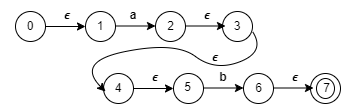
\includegraphics[width=0.45\textwidth]{./ressources/NDFA_ab.png}
    \caption{Automate fini non déterministe de l'arbre ".(a,b)"}
    \cite{ndfa_ab}
    \label{fig:ndfa_ab}
\end{figure}

Pour la règle de concaténation ".", nous avons ajouté une nouvelle transition $\epsilon$ entre l'état 3 (ancien état d'acceptation de l'AFND gauche) et l'état 4 (état de départ de l'AFND droit).

Le tableau suivant correspond à l'AFND du graphe \cite{ndfa_ab} :
\begin{figure}[h] % Utilisation de l'option [h] pour placer l'image ici
    \centering
    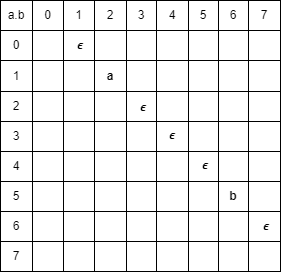
\includegraphics[width=0.38\textwidth]{./ressources/NDFA_ab.tab.png}
    \caption{Représentation sous forme de tableau de l'arbre ".(a,b)"}
    \cite{ndfa_tab_ab}
    \label{fig:ndfa__tab_ab}
\end{figure}

Pour les autres opérations, telles que l'étoile "*" et l'alternance "|", l'idée reste similaire, mais les règles diffèrent légèrement. Ces règles sont définies dans des méthodes d'une classe. Des appels de ces méthodes sont ensuite effectués jusqu'à atteindre la racine de l'arbre, afin de générer \textbf{un tableau à deux dimensions de caractères} représentant les transitions de l’automate .

\subsubsection{Convertir l’automate fini non déterministe en déterministe}
À partir de l'AFND, nous cherchons à éliminer toutes les transitions $\epsilon$ intermédiaires pour rendre l'automate déterministe en utilisant la méthode des sous-ensembles. Cette méthode commence par définir l'état de départ de l'AFD, qui est lui-même un ensemble d'états de l'AFND. Les états de l'AFD sont stockés dans des structures de type \textbf{HashSet} afin de garantir leur \textbf{unicité}.

En parcourant les sous-ensembles de tous les états de l'AFD, nous cherchons à déterminer si une transition existe pour chaque caractère d'entrée possible dans l'AFND.

Si c'est le cas, nous continuons le parcours tant que les transitions vers les autres états successeurs sont des transitions $\epsilon$. Ensuite, nous ajoutons les sous-ensembles des états successeurs comme nouveaux états de l'AFD. Le parcours s'arrête lorsqu'il n'y a plus d'états dans l'AFD nécessitant d'être parcourus.

Si l'un des sous-ensembles d'états de l'AFD contient l'état initial de l'AFND, cet état de l'AFD est défini comme état initial. De même, si un sous-ensemble contient l'état d'acceptation de l'AFND, cet état de l'AFD est défini comme état d'acceptation.

La structure de données utilisée pour stocker l'AFD est le \textbf{HashMap<String, HashMap<String, String>}. Les états de départ et d'acceptation sont stockés avec un \textbf{HashMap<String, Boolean>}. Ces choix de structures de données visent à optimiser l'allocation mémoire tout en permettant également une récupération rapide des états et des transitions grâce à son accès en temps constant O(1).

\subsubsection{Réduction de l'AFD (Minimisation)}
L'optimisation la plus courante pour un AFD est la \textbf{minimisation}. Réduire le nombre d'états tout en conservant les mêmes propriétés de reconnaissance du langage. Dans ce projet, on a utilisé un algorithme de partitionnement des états souvent appelé algorithme de Moore.

La première étape consiste à identifier les états atteignables à partir de l'état initial. Cette opération est réalisée en utilisant une exploration en largeur (BFS). Tous les états qui ne peuvent être atteints sont supprimés de l'automate, ce qui simplifie l'AFD en éliminant des états inutiles, rendant ainsi le calcul plus efficace, plus rapide et optimise l’utilisation de la mémoire. 

Dans le processus de partitionnement des états équivalents, on commence par diviser les états en deux groupes principaux : les \textbf{états finaux} et les \textbf{états non-finaux}, qui ne peuvent jamais être équivalents.

Par la suite, chaque groupe est progressivement subdivisé en fonction des transitions. Deux états sont dits équivalents s'ils ont les mêmes transitions vers des groupes identiques d'états. Pour cela, une méthode de signature est utilisée, où chaque état est caractérisé par la "signature" des états vers lesquels il se dirige. Si deux états partagent la même signature, ils sont considérés comme équivalents.

Cette étape se répète jusqu'à ce que les partitions ne puissent plus être subdivisées, assurant ainsi que chaque groupe contient des états totalement équivalents. Une fois les partitions stables identifiées, les états équivalents sont fusionnés. Cela se traduit par la création d’un mapping qui associe chaque ancien état à un état représentant l'ensemble des états équivalents. Cette fusion réduit le nombre total d’états dans l’automate tout en gardant son comportement.

À la fin du processus, un nouvel automate est construit en appliquant le mapping des états équivalents, créant ainsi un \textbf{AFD minimisé} qui contient moins d'états mais accepte le même langage que l’automate original.

\subsubsection{Recherche de motif}
Les étapes de recherche des motifs dans un fichier .txt donnée peuvent être réparties en 3 étapes:

\begin{itemize}
    \item Une méthode qui  prend une ligne de texte à partir d'une position donnée et vérifie si une sous-chaîne est acceptée par l'AFD .Le parcours commence à l’état initial et se déplace selon les transitions de l’automate, vérifiant chaque symbole. Si un état final est atteint, la sous-chaîne est acceptée.
    \item La méthode qui vérifie dans une ligne parcourt chaque sous-chaîne possible d’une ligne pour trouver des correspondances avec l’automate. Si une sous-chaîne est acceptée, la ligne est validée.
    \item On parcourt chaque ligne d’un fichier et applique la vérification. Les lignes contenant des sous-chaînes acceptées sont affichées avec leur numéro.
\end{itemize}

\subsection{Algorithme Knuth-Morris-Pratt (KMP)}
L'algorithme de Knuth-Morris-Pratt (KMP) est un algorithme de recherche de sous-chaîne dans une chaîne de caractères.

Cet algorithme utilise une technique de prétraitement pour créer un tableau d'indices de décalage (LPS - Longest Prefix Suffix), ce qui permet de sauter des comparaisons inutiles et d'optimiser la recherche. Il est basé sur l'idée de ne pas comparer les caractères qui ont déjà été comparés. Au lieu de cela, il utilise un tableau d'indices de décalage pour sauter les comparaisons inutiles.

Voici la méthodologie du déroulement de l’algorithme KMP :

\begin{itemize}
    \item Prétraitement du motif : Calculer le tableau LPS du motif. Ce tableau aide à déterminer jusqu'où le motif peut être décalé en cas de désaccord partiel lors de la recherche dans le texte.
    \item Recherche dans le texte : Parcourir le texte de manière linéaire tout en exploitant le tableau LPS pour éviter de revérifier les caractères qui correspondent déjà.
\end{itemize}

\newpage
\section{Test et Analyse de performance}

Pour la phase de test des algorithmes, nous mesurerons les temps d'exécution minimum, maximum et moyen de l'algorithme en fonction de différents motifs appliqués à un même texte. Le texte choisi est \textit{Pony Tracks} de Frederic Remington, récupéré sur le site \texttt{gutenberg.org}.

\subsection{Automate}

Pour l’automate, nous choisissons de faire deux tests. Le premier en utilisant des motifs RegEx et le deuxième en utilisant des motifs simples pour pouvoir les comparer avec l’algorithme Knuth-Morris-Pratt.

Les motifs RegEx utilisés pour ces tests sont : \texttt{"a|bc*"}, \texttt{"th(e|is)"}, \texttt{"ex\.*ple"}, \texttt{"\"[\^  " ]+\""} et \texttt{"t\.*t"}.

\begin{figure}[ht] % Utilisation de l'option [h] pour placer l'image ici
    \centering
    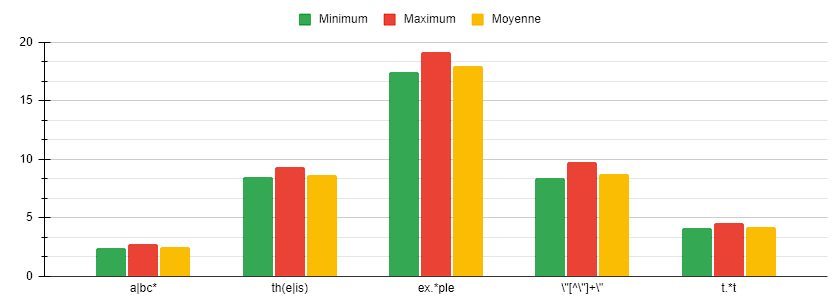
\includegraphics[width=1\textwidth]{./ressources/test_automate_regex.png}
    \caption{Diagramme des temps d'exécutions des RegEx avec l'algorithme Automate}
    \cite{test_automate_regex}
    \label{fig:test_automate_regex}
\end{figure}

Les résultats montrent les temps d'exécution d'un algorithme utilisant un automate pour effectuer des recherches de motifs à l'aide d'expressions régulières. Ces temps varient en fonction de la complexité de chaque motif. Par exemple, pour un motif simple comme \texttt{"a|bc*"}, les temps d'exécution restent assez bas, avec un minimum de 2,4012 ms, un maximum de 2,795 ms, et une moyenne de 2,4781 ms. En revanche, un motif plus complexe comme \texttt{"ex.*ple"} entraîne des temps d'exécution bien plus élevés, avec une moyenne de 17,9293 ms, ce qui suggère que les recherches impliquant des caractères génériques sont plus coûteuses en termes de performance.

D'autres motifs, comme \texttt{"th(e|is)"} et \texttt{"\"[\^ " ]+\""}, affichent des temps d'exécution intermédiaires, avec des moyennes respectives de 8,6313 ms et 8,7615 ms. Le motif \texttt{"t.*t"} se situe quant à lui dans une fourchette modérée, avec une moyenne de 4,2565 ms, montrant ainsi une bonne efficacité pour cette structure relativement simple.

Ces résultats illustrent l'impact de la complexité et de la longueur des motifs sur les performances de l'algorithme.

Pour les motifs plus simples, voici ceux qui ont été utilisés : \texttt{"war"}, \texttt{"shoot"}, \texttt{"queen"}, \texttt{"dolls"}, \texttt{"General Miles was"}, \texttt{"Lieutenant Casey"}, \texttt{"the queen's coronation"}, \texttt{"in the heart of the jungle"}, \texttt{"good encyclopædia"}, \texttt{"Hooick"}.

\newpage

\begin{figure}[ht] % Utilisation de l'option [h] pour placer l'image ici
    \centering
    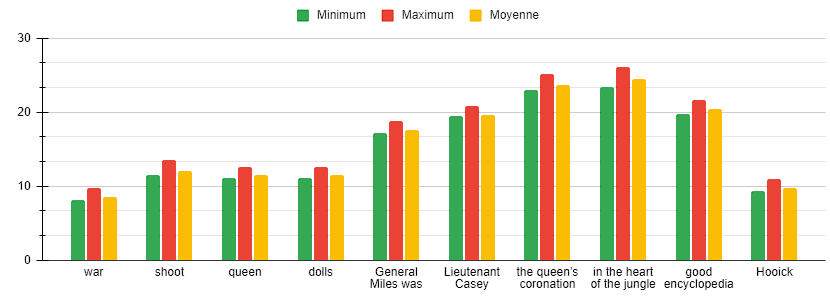
\includegraphics[width=1\textwidth]{./ressources/test_automate_motifs.png}
    \caption{Diagramme des temps d'exécutions des motifs simples avec l'algorithme Automate}
    \cite{test_automate_motif}
    \label{fig:test_automate_motif}
\end{figure}


Les résultats présentés montrent les temps d'exécution d'un algorithme qui utilise un automate pour rechercher des motifs dans des chaînes de texte. Les valeurs minimales, maximales et moyennes révèlent des variations notables en fonction de la longueur et de la complexité des chaînes. Par exemple, les chaînes courtes comme \texttt{"war"} enregistrent un temps d'exécution minimum de 8,1955 ms et un maximum de 9,7808 ms, avec une moyenne de 8,6151 ms.

En revanche, les chaînes plus longues et complexes, telles que \texttt{"in the heart of the jungle"} et \texttt{"the queen’s coronation"}, affichent des temps d'exécution beaucoup plus élevés, avec des moyennes respectives de 24,4647 ms et 23,7268 ms. Les autres chaînes se situent entre ces deux extrêmes, avec des moyennes variant de 9,8029 à 20,3826 ms.

Ces résultats mettent en évidence la variation significative des performances de l'algorithme en fonction de la taille et de la structure des chaînes, indiquant que l'automate est plus sensible aux chaînes longues et complexes.

\subsection{Algorithme Knuth-Morris-Pratt (KMP)}

Pour l'algorithme KMP, nous appliquons les mêmes motifs simples que ceux utilisés avec l'automate : \texttt{"war"}, \texttt{"shoot"}, \texttt{"queen"}, \texttt{"dolls"}, \texttt{"General Miles was"}, \texttt{"Lieutenant Casey"}, \texttt{"the queen's coronation"}, \texttt{"in the heart of the jungle"}, \texttt{"good encyclopædia"} et \texttt{"Hooick"}.

\begin{figure}[ht] % Utilisation de l'option [h] pour placer l'image ici
    \centering
    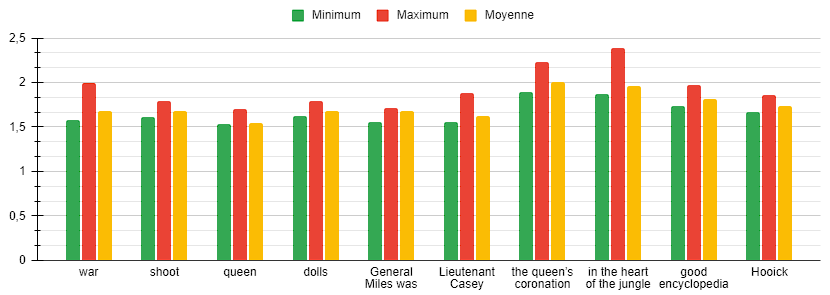
\includegraphics[width=1\textwidth]{./ressources/test_kmp_motifs.png}
    \caption{Diagramme des temps d'exécutions des motifs simples avec l'algorithme KMP}
    \cite{test_kmp_motif}
    \label{fig:test_kmp_motif}
\end{figure}

Les résultats présentés illustrent les temps d'exécution de l'algorithme KMP lorsqu'il est appliqué à diverses chaînes de texte. En examinant les temps d'exécution minimum, maximum et moyen, on peut évaluer les performances de l'algorithme dans différentes situations.

Dans l'ensemble, les temps moyens varient entre 1,5 et 2 ms, ce qui indique que l'algorithme offre une performance relativement stable. Les chaînes plus courtes ou simples, comme \texttt{"war"} et \texttt{"shoot"}, affichent des temps d'exécution plus bas, avec des moyennes avoisinant 1,68 ms.

En revanche, les chaînes plus longues ou complexes, telles que \texttt{"the queen’s coronation"} et \texttt{"in the heart of the jungle"}, montrent des temps d'exécution plus élevés, dépassant les 2 ms. Cette augmentation est due à la complexité croissante des motifs de recherche dans des chaînes plus longues, entraînant une légère dégradation des performances de l'algorithme, bien qu'il soit conçu pour optimiser les recherches. Les variations entre les temps minimum et maximum restent relativement faibles, ce qui témoigne de la robustesse et de la stabilité de KMP dans différentes configurations de chaînes.

\subsection{Comparaison}

La comparaison des temps d'exécution entre l'algorithme Knuth-Morris-Pratt (KMP) et un algorithme basé sur un automate révèle des différences notables en termes de performances, qui dépendent de la complexité des motifs et des chaînes analysées.

\subsubsection{Performances générales}
L'algorithme KMP se montre généralement plus rapide que l'automate dans presque tous les scénarios. Par exemple, pour des chaînes courtes comme \texttt{"war"}, KMP affiche une moyenne de 1,6832 ms, alors que l'automate nécessite 8,6151 ms. Cette tendance est corroborée pour la plupart des chaînes, avec des écarts significatifs. Par exemple :
\begin{itemize}
    \item Pour \texttt{"in the heart of the jungle"}, KMP prend en moyenne 1,9605 ms, tandis que l'automate atteint 24,4647 ms.
    \item Pour \texttt{"the queen’s coronation"}, les temps moyens sont respectivement de 2,0063 ms pour KMP et 23,7268 ms pour l'automate.
\end{itemize}
Ces différences illustrent que KMP est bien plus rapide pour des recherches classiques, surtout lorsque les motifs sont simples ou que les chaînes sont courtes.

\subsubsection{Impact de la complexité des motifs}
En ce qui concerne la recherche avec des expressions régulières, l'automate révèle une sensibilité marquée à la complexité des motifs. Par exemple, pour un motif tel que \texttt{"a|bc*"}, l'automate présente un temps moyen de 2,4781 ms, ce qui le rend comparable à KMP sur de petites chaînes. Toutefois, dès que les motifs deviennent plus complexes, comme \texttt{"ex.*ple"}, le temps d'exécution de l'automate augmente considérablement, atteignant en moyenne 17,9293 ms.

En revanche, KMP est conçu pour maintenir des performances stables avec des motifs plus simples, sans nécessiter de traitements avancés pour des correspondances plus complexes comme les expressions régulières.

\subsubsection*{Stabilité des temps d'exécution}
Un autre aspect important est la stabilité des deux algorithmes. Les variations entre les temps minimum et maximum sont nettement plus marquées pour l'automate, surtout avec des chaînes longues et complexes. Par exemple, pour \texttt{"in the heart of the jungle"}, l'automate présente des temps variant entre 23,3693 et 26,1084 ms, tandis que KMP oscille entre 1,8659 et 2,3912 ms. Cela montre que KMP est plus prévisible et constant dans ses temps d'exécution, alors que l'automate peut subir des fluctuations significatives selon les cas d'utilisation.

\subsubsection{Conclusion}
En résumé, l'algorithme KMP surpasse largement l'algorithme basé sur un automate en termes de rapidité et de stabilité, particulièrement pour les chaînes courtes ou simples. Bien que l'automate soit mieux adapté à la gestion de motifs complexes avec des expressions régulières, il souffre de performances nettement inférieures, notamment pour les chaînes plus longues. En conséquence, KMP s'avère être un choix plus approprié dans des contextes où la rapidité est essentielle et les motifs sont simples. En revanche, l'automate trouve son utilité dans des situations où les motifs sont plus complexes, bien que cela entraîne un coût en temps plus élevé.


\newpage
\section{Analyse critique}
La sélection entre l'algorithme KMP et la méthode d’Aho-Ullman dépend des besoins spécifiques de l’application, notamment du nombre de motifs à rechercher et de l’environnement dans lequel l’application sera utilisée.

La méthode Aho-Ullman est rapide dans les contextes où plusieurs motifs doivent être recherchés en une seule passe. Elle est donc très performante dans des scénarios de filtrage, tels que les moteurs de recherche. Cependant, pour atteindre cette performance, l’implémentation de l’algorithme requiert une allocation mémoire conséquente. La construction de l’automate a une complexité algorithmique de \( O(m \cdot k) \), où \( m \) est la longueur totale des motifs et \( k \) est le nombre de motifs. En revanche, la recherche dans le texte est linéaire, avec une complexité de \( O(n + z) \), où \( n \) est la longueur du texte et \( z \) est le nombre de correspondances trouvées. Ainsi, la méthode Aho-Ullman présente une complexité globale de \( O(m \cdot k + n + z) \). Pour utiliser cette méthode efficacement, il est nécessaire d’avoir un environnement souple en termes de stockage.

L’algorithme KMP, en revanche, est plus adapté aux applications où le motif recherché est unique. Il est utile, par exemple, pour valider une sous-chaîne dans des données ou analyser des séquences avec des motifs fréquents. Cet algorithme est simple et léger en termes d’espace mémoire. Il présente une complexité linéaire \( O(m) \) pour le prétraitement du motif (par rapport à sa longueur \( m \)), et une complexité linéaire \( O(n) \) pour la recherche dans le texte (par rapport à sa longueur \( n \)), pour une complexité totale de \( O(n + m) \). KMP est donc idéal dans des contextes où les ressources sont limitées.

Au cours de l'implémentation de ce projet, nous avons constaté que la mise en œuvre de la méthode Aho-Ullman est bien plus complexe que celle de l’algorithme KMP. Dans les contextes où la recherche de motif est effectuée motif par motif, il est préférable d’utiliser KMP.

Pour la méthode Aho-Ullman, nous avons pris en compte uniquement les opérateurs ``*'', ``|'', ``.'', ainsi que les lettres et concaténations. Il serait possible d’étendre le projet en ajoutant d'autres opérateurs d'expressions régulières, tels que ``?'', ``\$'', ``+'', etc.

\newpage
\section{Conclusion}
Le choix entre KMP et Aho-Ullman dépend d'un compromis entre performance, complexité d'implémentation et contraintes mémoires. Pour des recherches multiples et complexes, Aho-Ullman est un excellent choix. Pour des recherches simples et rapides, KMP est souvent suffisant.

Ce projet nous a permis d'approfondir notre compréhension des algorithmes de recherche de motifs et de mettre en pratique nos connaissances théoriques. La construction de l'automate d'Aho-Ullman nous a familiarisés avec les concepts de théorie des graphes, tandis que l'analyse de la complexité algorithmique de chaque méthode a souligné l'importance du choix des structures de données adaptées.

En somme, ce travail a mis en évidence la richesse et la diversité des approches algorithmiques pour un problème aussi fondamental que la recherche de motifs dans des textes.

\newpage
\bibliographystyle{unsrt}
\bibliography{references}
\end{document}